{\bf Problem 4: Answers}

\begin{enumerate}
    \item
	    $\lambda_1$: 5.148333441485338 \\
	    $\lambda_2$: 3.7299894906022617 \\
	    $\lambda_{10}$: 1.250010757212031 \\
	    $\lambda_{30}$: 0.36492647617793883 \\
	    $\lambda_{50}$: 0.16962131566853172 \\
	    $\sum_{i=1}^d \lambda_i$: 52.83384400094484
    \item Show a general formula for the rank-$k$ PCA approximation of $x$.
	\begin{align*}
	    \Sigma &= \frac{1}{n} \left( X_{\textrm{train}} - \mathbf{1} \mu^T \right)^T \left( X_{\textrm{train}} - \mathbf{1} \mu^T \right) \\
		&= \frac{1}{n} \left( U S V^T \right)^T \left( U S V^T \right) \tag*{Substitute SVD of $X_{\textrm{train}} - \mathbf{1} \mu^T$} \\
		&= \frac{1}{n} V S U^T U S^T V^T \\
		&= \frac{1}{n} V S^2 V^T \\
		&= \frac{1}{n} \left( X_{\textrm{train}} - \mathbf{1} \mu^T \right) \left( X_{\textrm{train}} - \mathbf{1} \mu^T \right) V \\
		&= \frac{1}{n} V S^2 \\
		&= \frac{1}{n} V D
	\end{align*}
	Now consider that since $S$ is a diagonal matrix,
	    \begin{equation*}
		S^2 = 
		    \begin{bmatrix}
			s_1^2 & 0 & 0 & ... \\
			0 & s_2^2 & ... & 0 \\
			0 & 0 & ... & ... \\
			0 & 0 & ... & 0
		    \end{bmatrix}	
	    \end{equation*}
	Which implies that 
	    \begin{equation*}
		\frac{1}{n} D = 
		    \begin{bmatrix}
			\frac{1}{n} d_1 & 0 & 0 & ... \\
			0 & \frac{1}{n} d_2 & ... & 0 \\
			0 & 0 & ... & ... \\
			0 & 0 & ... & 0
		    \end{bmatrix}	
	    \end{equation*}
	Therefore, let $\lambda_i = \frac{1}{n} d_i$ where $\lambda_i$ is the $i$-th eigenvalue of $V$
	    \begin{align*}
		\Sigma V &= \frac{1}{n} V D \\
			&= V
			\begin{bmatrix}
			    \lambda_1 & 0 & 0 & ... \\
			    0 & \lambda_2 & ... & 0 \\
			    0 & 0 & ... & ... \\
			    0 & 0 & ... & 0
			\end{bmatrix} \\
		\Sigma v_i &= \lambda_i v_i
	    \end{align*}
	So $\left( X_{\textrm{train}} - \mathbf{1} \mu^T \right)$ where $x_i \in \R$ can be projected onto $k$ dimensions by using the first $k$ eigenvectors of $V$ to compute the minimum reconstruction error. 
	Thus, a general formula for the rank-$k$ PCA approximation for $x$ can be written $$ \bar{x} = V_k V_k^T \left(x_i - \mu^T \right) + \mu $$
    \item See Figures 4 and 5
	\begin{figure}[h!]
	    \centering
	    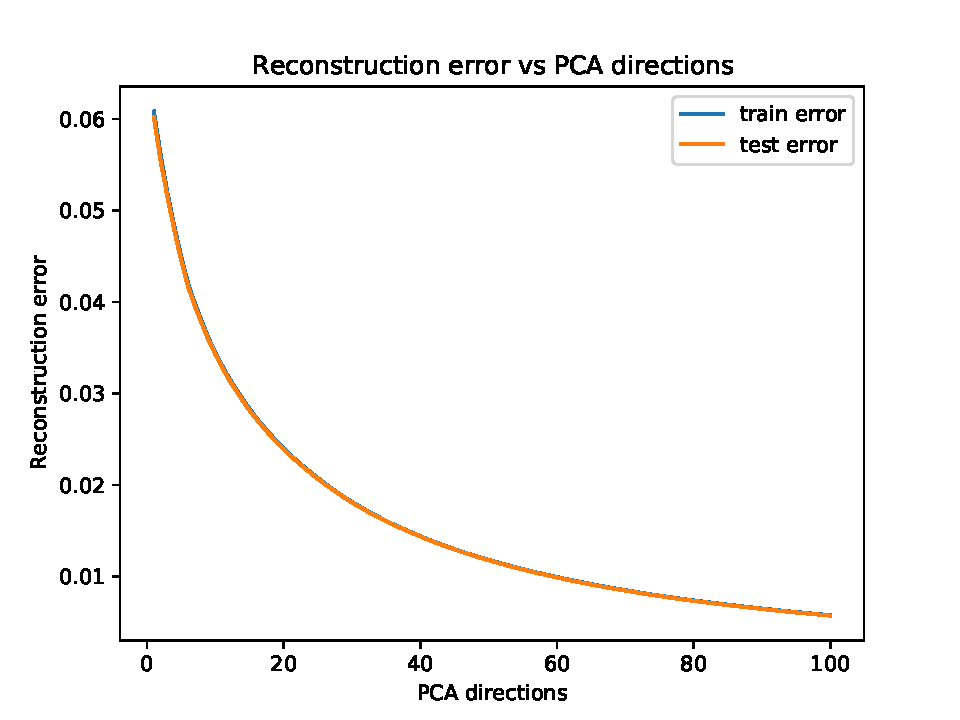
\includegraphics[width=0.8\linewidth]{../figures/a4_re.pdf}
	    \caption{}
	\end{figure}
	\begin{figure}[h!]
	    \centering
	    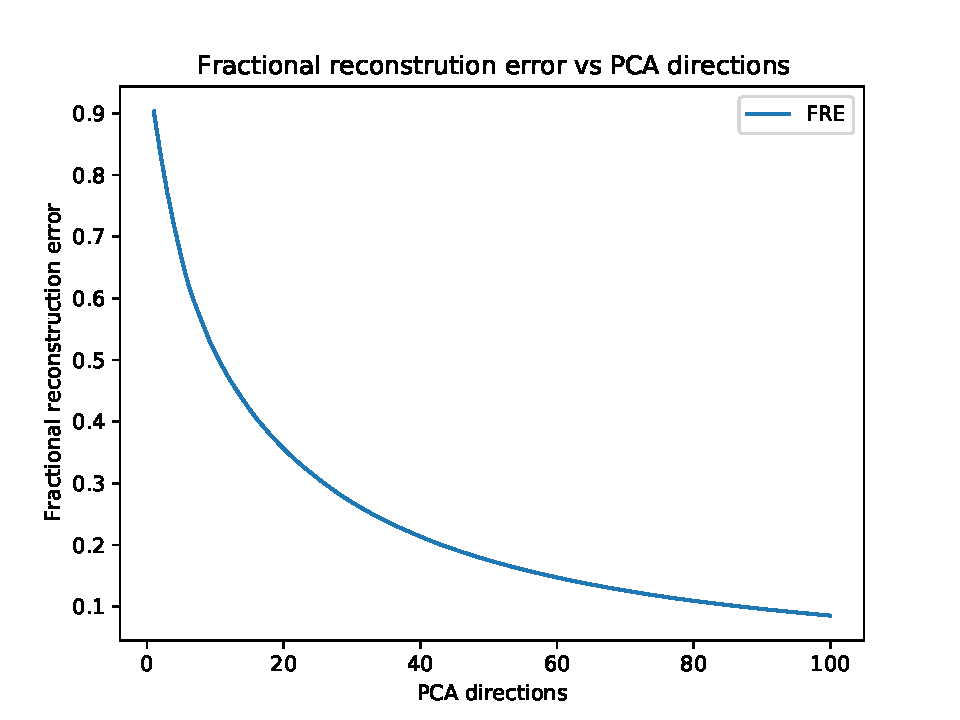
\includegraphics[width=0.8\linewidth]{../figures/a4_fre.pdf}
	    \caption{}
	\end{figure}
    \item See Figure 6. These represent the first 10 eigenvectors in the single value decomposition of the sample covariance of training examples. They correspond to the most significant entries in the training dataset and so contain overlapping, repeated, and missing digits.
	\begin{figure}[h!]
	    \centering
	    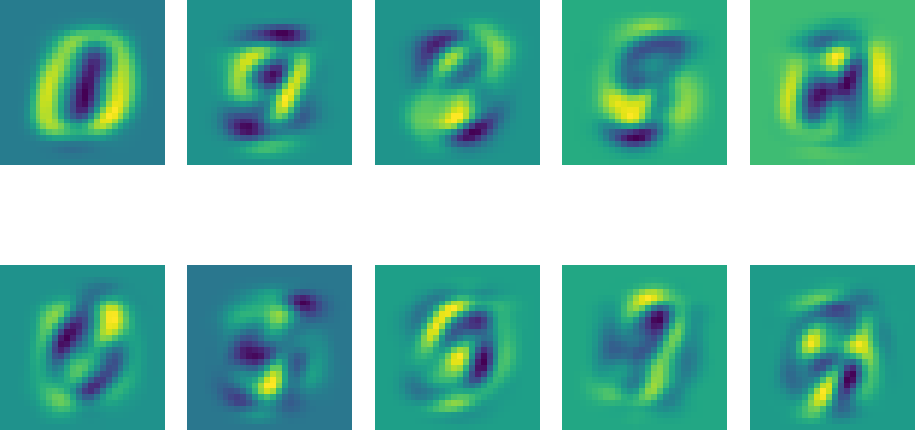
\includegraphics[width=0.8\linewidth]{../figures/a4_eigenvectors.pdf}
	    \caption{}
	\end{figure}
    \item See Figure 7. Increasing k improves the fidelity of the reconstruction. 
    \begin{figure}[h!]
	    \centering
	    \caption{}
	    
\includegraphics[width=0.6\linewidth]{../figures/a4_actual.pdf}
	    \caption*{Actual}
	    
\includegraphics[width=0.6\linewidth]{../figures/a4_recon_5.pdf}
	    \caption*{k=5}
	    
\includegraphics[width=0.6\linewidth]{../figures/a4_recon_15.pdf}
	    \caption*{k=15}
	    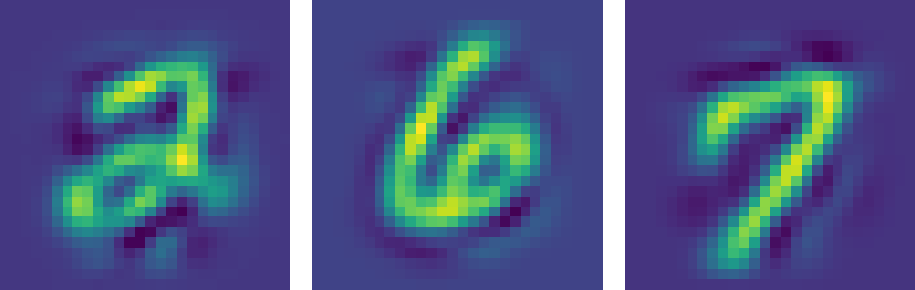
\includegraphics[width=0.6\linewidth]{../figures/a4_recon_40.pdf}
	    \caption*{k=40}
	    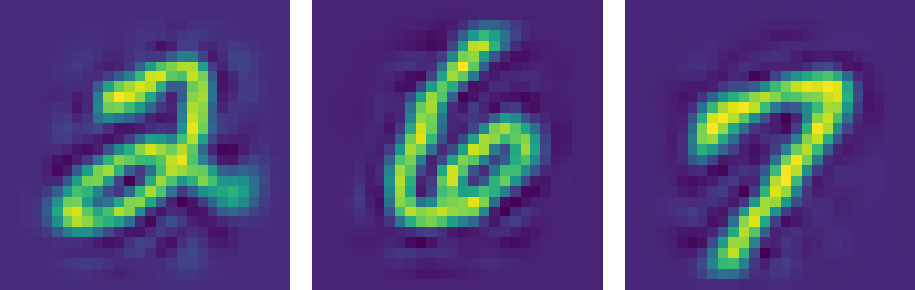
\includegraphics[width=0.6\linewidth]{../figures/a4_recon_100.pdf}
	    \caption*{k=100}
	\end{figure}
\end{enumerate}

{\bf Problem 4: Code}
\begin{quote}
    \lstinputlisting[language=Python]{../code/a4.py}
\end{quote}
